%-----------------------------------------------------------------
%	TOOLS AND DATA
%	!TEX root = ./../main.tex
%-----------------------------------------------------------------
\section{Tools and data}
% SHOULD INCLUDE:
%	Data life-cycle description
%	Tools and data used
%	Legal (license of the data) and ethical issues (not appliable)

\subsection{Data description}

\begin{table}[H]
	\centering
	\label{tab:city-list}
	\begin{tabular}{l l l l l}
	\toprule
	\toprule
	City          & State          & Region    & Life Cycle            & License \\
	\midrule
	Atlanta       & Georgia        & South     & \numrange{2009}{2016} &         \\
	Austin        & Texas          & South     & \numrange{2014}{2015} &         \\
	Baltimore     & Maryland       & Northeast & \numrange{2012}{2016} &         \\
	Chicago       & Illinois       & Midwest   & \numrange{2001}{2016} &         \\
	Dallas        & Texas          & South     & \numrange{2014}{2016} &         \\
	Detroit       & Michigan       & Midwest   & \numrange{2011}{2014} &         \\
	Los Angeles   & California     & West      & \numrange{2010}{2016} &         \\
	Metro Area    & Washington, DC & Northeast & \numrange{2008}{2016} &         \\
	Minneapolis   & Minnesota      & Midwest   & \numrange{2010}{2016} &         \\
	New York City & New York       & Northeast & \numrange{2014}{2016} &         \\
	Philadelphia  & Pennsylvania   & Northeast & \numrange{2006}{2016} &         \\
	Portland      & Oregon         & West      & \numrange{2015}{2016} &         \\
	San Francisco & California     & West      & \numrange{2003}{2016} &         \\
	Seattle       & Washington     & West      & \numrange{2009}{2016} & \\
	\bottomrule
	\end{tabular}
	\caption{Caption here}
\end{table}

\begin{figure}[H]
	\centering
	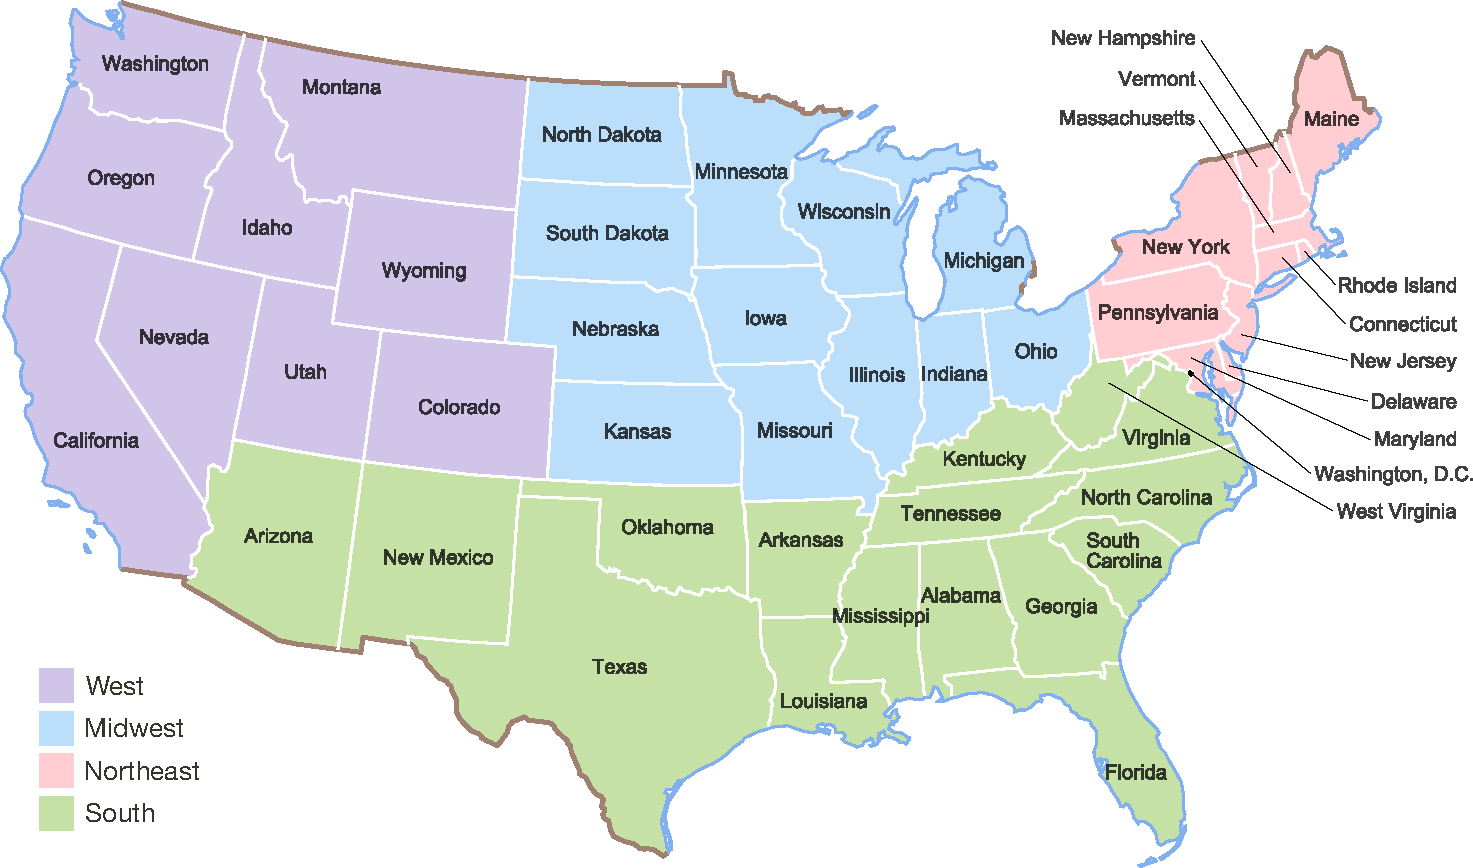
\includegraphics[width=\textwidth]{./images/us-map}
	\caption{Caption here}
	\label{fig:us-map}
\end{figure}


\subsection{Data mining process}


